%=============================================================================
% Thesis Template in LaTex
%
% File:  07-Schlussfolgerung.tex -- Schlussfolgerung und Ausblick
% Author(s): Cyrano Golliez <golliezc@student.ethz.ch>
%
% Creation:  27 Jan 2014
% Time-stamp: <Tue 2013-08-13 20:14 juergen>
%
% Copyright (c) 2014 Infrastructure Management Group (IMG)
%               http://ibi.ethz.ch
%
% More information on LaTeX: http://www.latex-project.org/
%=============================================================================

\chapter{Schlussfolgerung und Ausblick}
\label{chap:Schlussfolgerung}


Basierend auf den in Kapitel \ref{chap:Resultate} dargestellten Resultaten und der in Kapitel \ref{chap:Diskussion} durchgeführten Diskussion, ist die Variante 2 die optimale Verbesserung der Verkehrssituation in Uster. 

Unter den in Abschnitt \ref{sec:Kostenstruktur} getroffenen Annahmen und der unter Abschnitt \ref{subsec:Modellierung} modellierten Veränderungen des Mobilitätsbedarfes, ergibt sich, dass sich die Mehrkosten durch den Bau der Variante 2 gegenüber Variante 1 bei einer Betrachtung der Gesamtkosten über den Zeitraum von 40 Jahren, lohnen würden. Insbesondere unter der in Kapitel \ref{chap:Diskussion} durchgeführten, Betrachtung der Reisezeitkosten ergibt sich eine eindeutige Lösung zur Optimierung des Bahnübergangs Brunnenstrasse. Die Variante 2 ist nicht nur in ökologischer Hinsicht der Variante 1 überlegen, sondern auch im ökonomischen Sinne.

Die höheren Investitions- und Wartungskosten der Variante 2 rechnen sich demnach im Vergleich zur Variante 1, bei einer Betrachtung der Situation über 40 Jahre. Die Variante 3, die weitaus höhere Investitionskosten verursachen würde, lohnt sich, nach der in Kapitel \ref{chap:Resultate} und Kapitel \ref{chap:Diskussion} durchgeführten Diskussion der Risiken, aufgrund der höheren Reisezeitkosten, die infolge der verlängerten Wartezeit entstehen, nicht. \\
Ausser in der vierten Parameterauswahl der Sensitivitätsanalyse, in der die zu erwartende Reisezeit verändert wird, kann die Variante 3, aufgrund der höheren Gesamtkosten, als optimale Variante ausgeschlossen werden. Somit lohnen sich die Mehrkosten der Variante 3 nicht.

Anzumerken ist, dass sich die Ergebnisse bei der Berücksichtigung weiterer Interessengruppen sowie einer komplexeren Modellierung der Einflussfaktoren auf das DTV, verändern könnten. Aufgrund der begrenzten Möglichkeiten, die mir im Rahmen dieser Projektarbeit zur Beurteilung der Situation zur Verfügung standen, konnte ich nicht alle relevanten Faktoren in der Entscheidungsfindung berücksichtigen. Das sollte im Rahmen einer erweiterten Studie zur Situation am Bahnübergang Brunnenstrasse erfolgen.

Um die Situation am Bahnübergang vollständig abzubilden, müssen die Fussgänger und der ÖV miteinbezogen werden. Insbesondere der ÖV hat grosses Interesse an der zukünftigen Entwicklung des Bahnübergangs, da alle Busse, um die Gleisanalage zu queren, den Bahnübergang Brunnenstrasse nutzen. Zusätzlich müsste, um die effektive Verkehrssituation vor Ort in den Entscheidungsprozess miteinzubeziehen, eine Verkehrssimulation durchgeführt werden. So könnte im Fall der Variante 3 die entstehende Wartezeit aufgrund des Ampelsystems exakter bestimmt werden sowie könnten die Variante auf ihre Gebrauchstauglichkeit untersucht werden. 

Zu Beginn des von mir durchgeführten Problemlösungsprozesses, habe ich zur Vereinfachung die beteiligten Personen auf die in Abschnitt \ref{subsec:Gruppen} definierten Interessensgruppen reduziert, um im gegeben Zeitrahmen eine ansprechende Lösung erarbeiten zu können. 
Eine Aufteilung der Kosten nach den verschiedenen Interessensverbänden wäre im Rahmen der Diskussion sehr aufschlussreich gewesen. Da die die Situation und die Möglichkeiten die mir für die Modellierung zur Verfügung standen zur Folge haben, dass die Reisezeitkosten den gesamten Risikovergleich der Varianten bestimmten, habe ich im Rahmen der Diskussion der Ergebnisse auf diese Unterteilung verzichtet. Es wäre jedoch sehr interessant, im Rahmen der weiteren Prüfung der Varianten, eine vertieftere Beurteilung der Nutzer- und Besitzerkosten durchzuführen.

Hinsichtlich der zukünftigen Entwicklung der Mobilität wird das Fahrrad voraussichtlich auch auf Strecken bis zu 30km eine entscheidende Rolle bei der Verkehrsmittelwahl spielen. Aufgrund dessen und in Anbetracht der Bestrebungen der Stadt Uster, ein Zentrum von regionaler Bedeutung zu werden, ist die Förderung des ökologischen und zukunftsorientierten Langsamverkehrs unerlässlich und insbesondere im Rahmen einer nachhaltigen Stadtentwicklung voranzutreiben. \\
So wäre eine Erweiterung der geplanten Veloinfrastruktur entlang der Pfäffikerstrasse bis zum Spital sowie entlang der Bahnhofstrasse bis zum Sternenplatz im Rahmen einer vertiefen Untersuchung zu berücksichtigen. Eine mögliche Variante einer solchen Veloschnellroute könnte anhand des Beispiels der Radschnellwege von Kopenhagen erstellt werden, die sich in Dänemark bereits bewährt und das Pendeln mit dem Velo leichter und sicherer gemacht haben.  \\
Insbesondere unter Anbetracht der aktuellen Situation mit CoVid-19, in der das Velo eine Renaissance erlebt, muss der Ausbau und die Förderung der innerstädtischen Langsamverkehrsnetze vorangetrieben werden.

Nichtsdestotrotz ist, um eine nachhaltige Verbesserung der Verkehrslage in Uster zu erreichen, eine Berücksichtigung der weiteren Schwachstellen des Ustemer Verkehrsnetzes unerlässlich. Insbesondere die zukünftige Entwicklung des Nüsslikreisel sowie der Zürichstrasse haben einen grossen Einfluss auf die Stadtentwicklung. Hinzu kommt, dass die Optimierung eines Teilstücks einer bestehenden Infrastruktur nur dann erfolgen sollte, wenn die Einflüsse auf die umliegenden Systeme berücksichtigt werden. So muss, um Uster nachhaltig zu verbessern, nicht nur das Velonetz ausgebaut sondern das gesamte Verkehrskonzept der Stadt überarbeitet werden. 

\paragraph{Ausblick}

Die von mir vorgeschlagenen Schritte, die Uster in der nächsten Zeit tätigen soll, sind in der nachfolgenden Abbildung \ref{img:UsterFuture} dargestellt. \\
So ergibt sich einerseits, wie ausführlich besprochen, der Weg, die Variante 2 in Betracht zu ziehen und die weiteren Schritte dementsprechend einzuleiten, wie zum Beispiel der Beginn einer Detailstudie oder aber bereits der Start des Planungsprozesses. Der zweite Weg der sich der Stadt Uster anbietet, ist eine  Hauptstudie, wodurch infolge der ausführlichen Prüfung der Situation, entweder die Wahl der optimalen Variante bestätigt oder aber eine andere Variante als optimal bestimmt wird. Die letzte Möglichkeit, die sich der Stadt Uster bietet, ist die Option: Variante 1 - "nichts zu machen", wobei für relativ wenig Geld die Verkehrssicherheit marginal erhöht jedoch über einen Zeitraum von vierzig Jahren hohe Mehrkosten generiert wird.

\begin{figure}[h!]
	\centering
	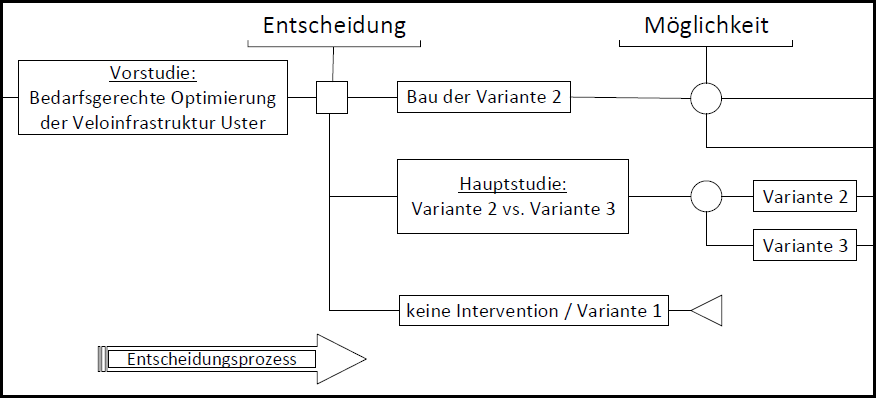
\includegraphics[width=\textwidth]{figures/f-07-01-EntscheidungsprozessUster}
	\caption[Entscheidungsprozess der Stadt Uster]{Möglicher Entscheidungsprozess der Stadt Uster für die nähere Zukunft}
	\label{img:UsterFuture}
\end{figure} 






% ===========================================================================
% EOF
%

%%% Local Variables:
%%% mode: latex
%%% TeX-master: "../main"
%%% End:
